\section{アプローチ11：身体向きベクトルの交差判定に基づく前後跨ぎグループ検出手法}

\subsection{手法の概要}
アプローチ10までの「距離および幾何的な列線への横並び判定」のみでは、壁際に寄って前後で会話をするカップルや、部活動等で前後複数列に跨がりながら対話するグループ、あるいは先に列に並んでいた連れに後から合流して並ぶケースなど、待機列特有の前後跨ぎグループを識別できないという課題が存在した。

アプローチ11では、スマートフォン操作等による下向きの視線変化の影響を避けるため顔の向きではなく「身体の向き（身体ベクトルの延長線）」を採用し、距離情報に加えて身体向きベクトルの交差角および交点距離を組み合わせたグループ判定アルゴリズム（\texttt{groupByOrientation.ts}）を導入した。

本アプローチにおける判定ロジックおよびモジュール構造の拡張仕様は以下の通りである。

\begin{itemize}
    \item \textbf{身体ベクトルの延長線交差判定}：
    待機列内で前後（隣接する前後のグループ間）に位置する人物ペアに対し、それぞれの持っている映像内身体向きベクトルの延長線が交差する角度を閾値によって評価する。
    \item \textbf{交点距離による誤判定防止}：
    ベクトルが交差する場合であっても、その交点が一定以上離れているケース（例：比較している2人のバウンディングボックス横幅平均値の2倍以上の距離）は、視線・身体が互いに向かい合っていないとみなしてグループ化から除外する。
    \item \textbf{連れ判定の波及効果}：
    横並びグループ内の誰か1人でも、前後列のグループに所属する人物と上記の身体向き条件を満たした場合、その前後グループ全体を同一の「連れ（グループ）」として拡張統合する。
    \item \textbf{モジュール構成}：
    \texttt{getGroups/groupPeople/} ディレクトリ内の \texttt{index.ts} に身体向きによる判定フローを追加し、独立した判定モジュールとして \texttt{groupByOrientation.ts} を新規作成・配置した。
\end{itemize}

\subsection{実験結果およびアプローチ10との比較・課題}

\subsubsection{実験結果}
静止画を入力データとして検証を行った際の実験結果を表\ref{tab:approach11_image_results}に示す。
なお、いずれの実験結果においても、緑色のバウンディングボックスは検出された人物、赤色のバウンディングボックスは同定されたグループを示している。

\begin{table}[H]
  \centering
  \small
  \caption{アプローチ11：実験結果の比較（静止画）}
  \label{tab:approach11_image_results}
  \adjustbox{max width=\textwidth}{%
  \begin{tabular}{|c|c|c|c|c|}
    
    \hline

      & \begin{tabular}{c} 前アプローチの \\ 検出結果 \end{tabular}
      & 検出結果
      & \begin{tabular}{c} 検出された \\ グループ数 \end{tabular}
      & 実際のグループ数との差 \\
    
    \hline
    
    $\vcenter{\hbox{標準状態}}$ &
      $\vcenter{\hbox{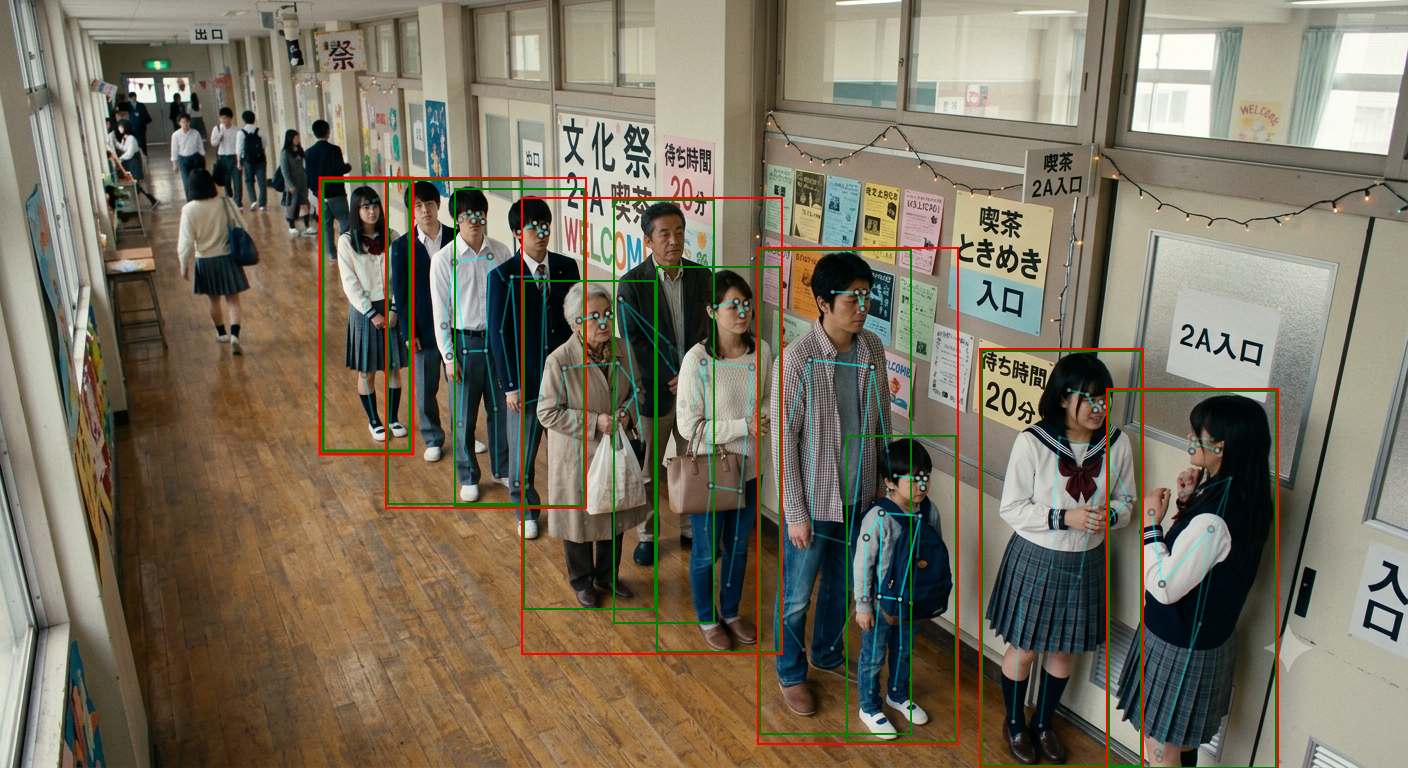
\includegraphics[width=0.25\textwidth]{experiment/results/approach_10_change_detection_model/standard/detection_outputs/annotated_images/t_001s.png}}}$ &
      $\vcenter{\hbox{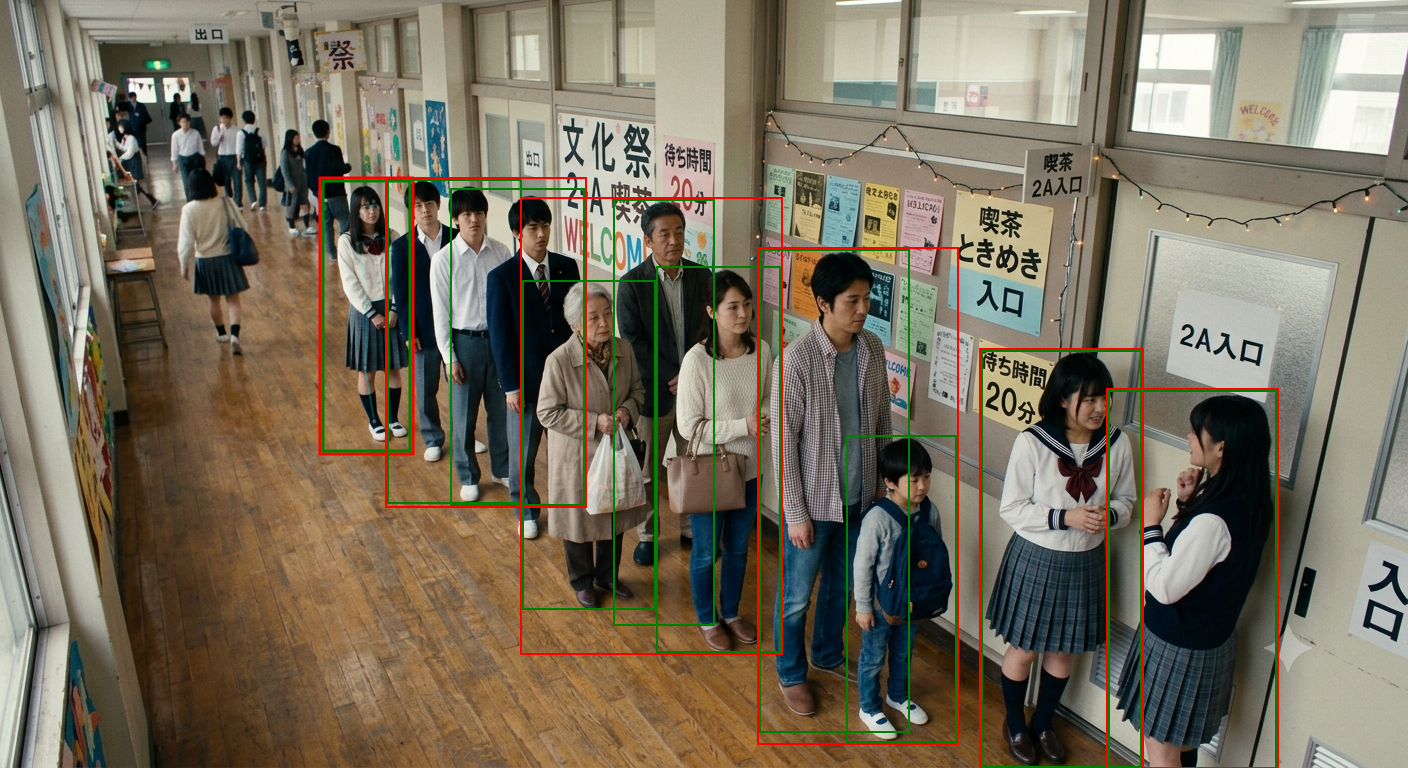
\includegraphics[width=0.25\textwidth]{experiment/results/approach_11_vector_orientation_grouping/standard/detection_outputs/annotated_images/t_001s.png}}}$ &
      \jsonlen{experiment/results/approach_11_vector_orientation_grouping/standard/detection_outputs/labels/t_001s.json} &
      % 符号と数値
        \ifnum\numexpr \jsonlen{experiment/results/approach_11_vector_orientation_grouping/standard/detection_outputs/labels/t_001s.json} - \gtstandard\relax>0 +\fi\the\numexpr
        \jsonlen{experiment/results/approach_11_vector_orientation_grouping/standard/detection_outputs/labels/t_001s.json} - \gtstandard\relax \\
    
    \hline
    
    $\vcenter{\hbox{密集状態}}$ &
      $\vcenter{\hbox{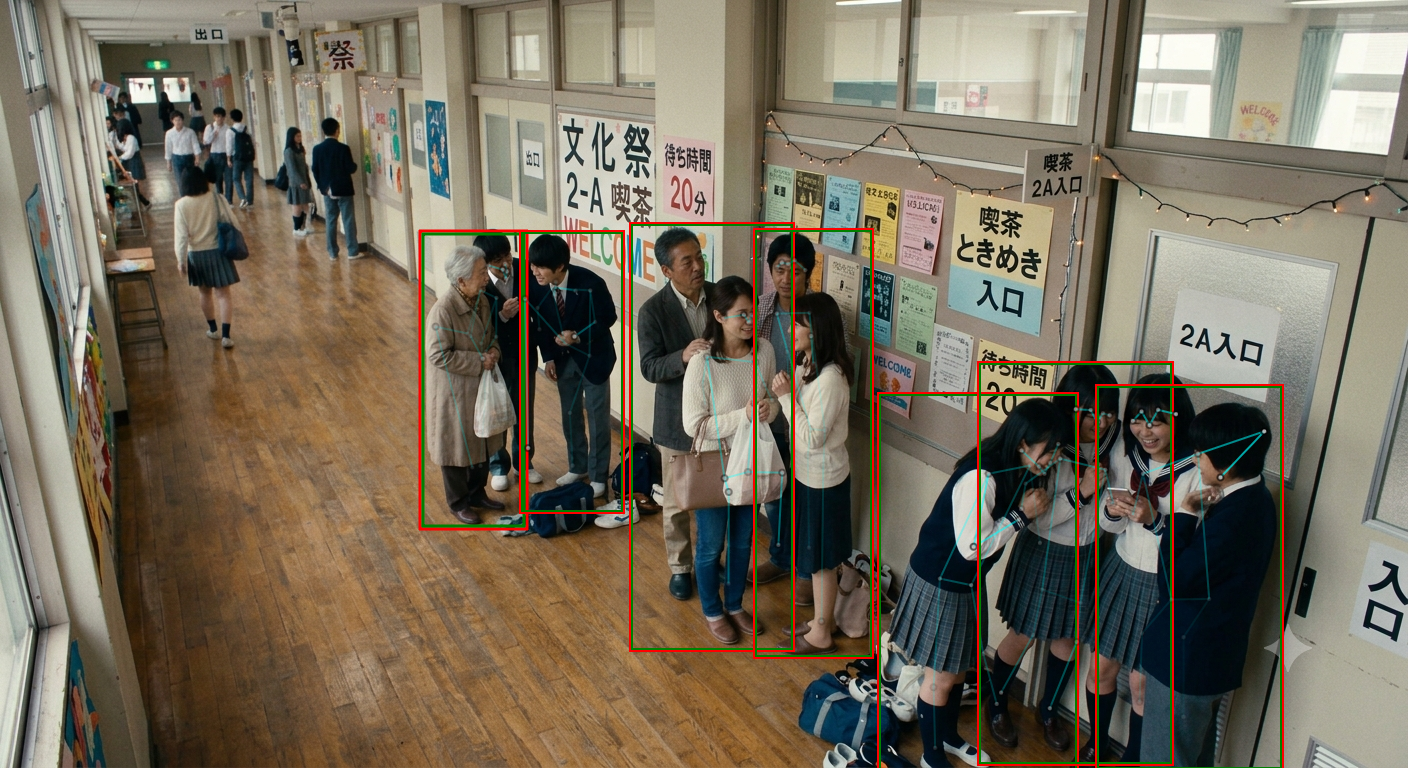
\includegraphics[width=0.25\textwidth]{experiment/results/approach_10_change_detection_model/crowded/detection_outputs/annotated_images/t_001s.png}}}$ &
      $\vcenter{\hbox{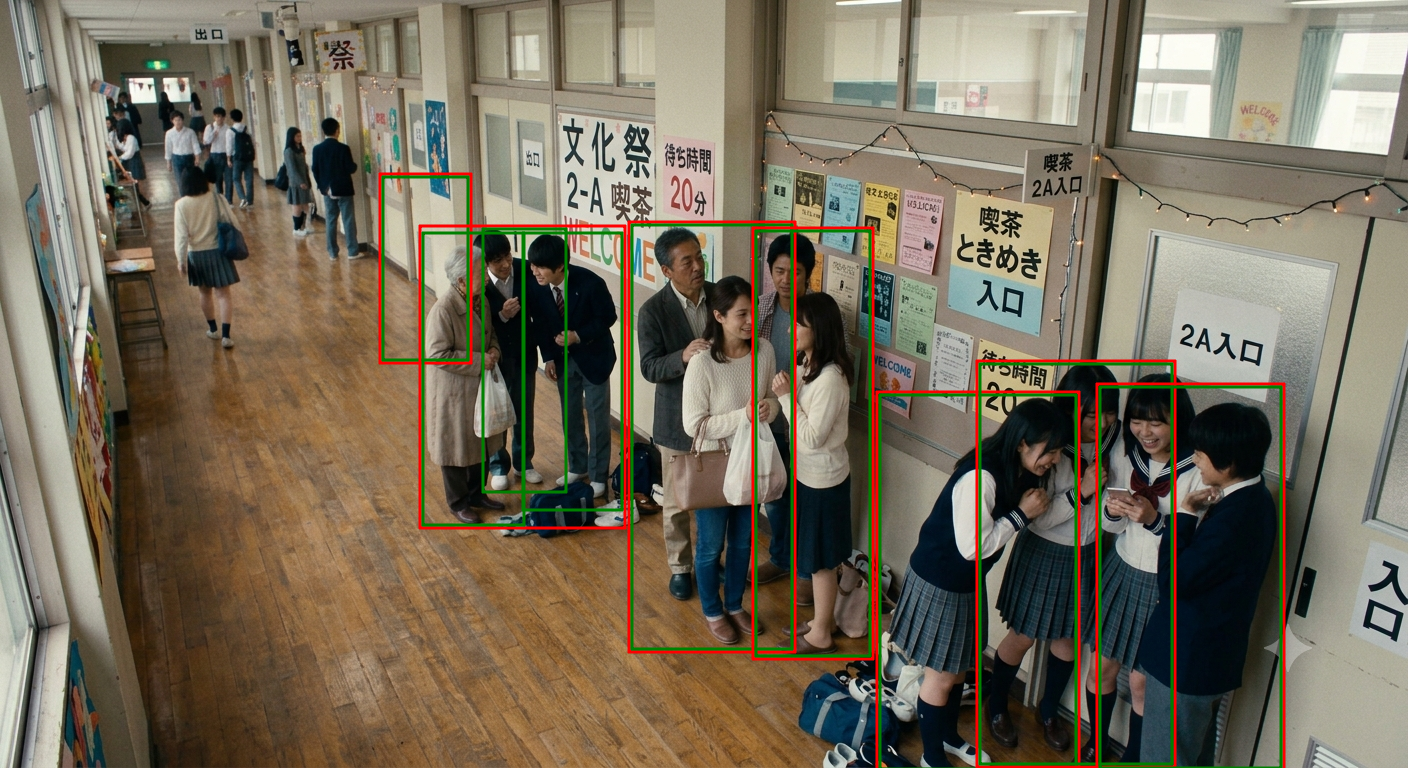
\includegraphics[width=0.25\textwidth]{experiment/results/approach_11_vector_orientation_grouping/crowded/detection_outputs/annotated_images/t_001s.png}}}$ &
      \jsonlen{experiment/results/approach_11_vector_orientation_grouping/crowded/detection_outputs/labels/t_001s.json} &
      % 符号と数値
        \ifnum\numexpr \jsonlen{experiment/results/approach_11_vector_orientation_grouping/crowded/detection_outputs/labels/t_001s.json} - \gtcrowded\relax>0 +\fi\the\numexpr
        \jsonlen{experiment/results/approach_11_vector_orientation_grouping/crowded/detection_outputs/labels/t_001s.json} - \gtcrowded\relax \\
    
    \hline
    
    $\vcenter{\hbox{非組織群集}}$ &
      $\vcenter{\hbox{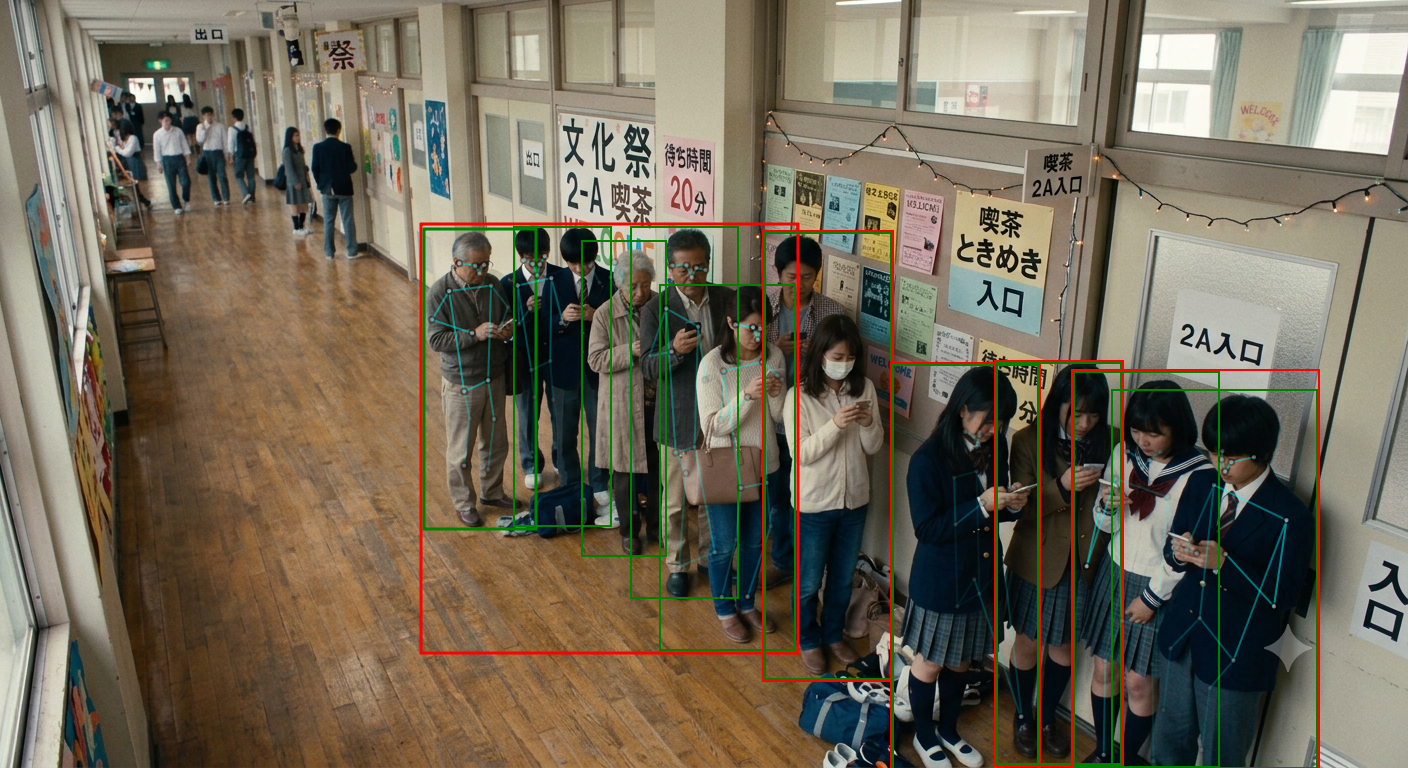
\includegraphics[width=0.25\textwidth]{experiment/results/approach_10_change_detection_model/strangers/detection_outputs/annotated_images/t_001s.png}}}$ &
      $\vcenter{\hbox{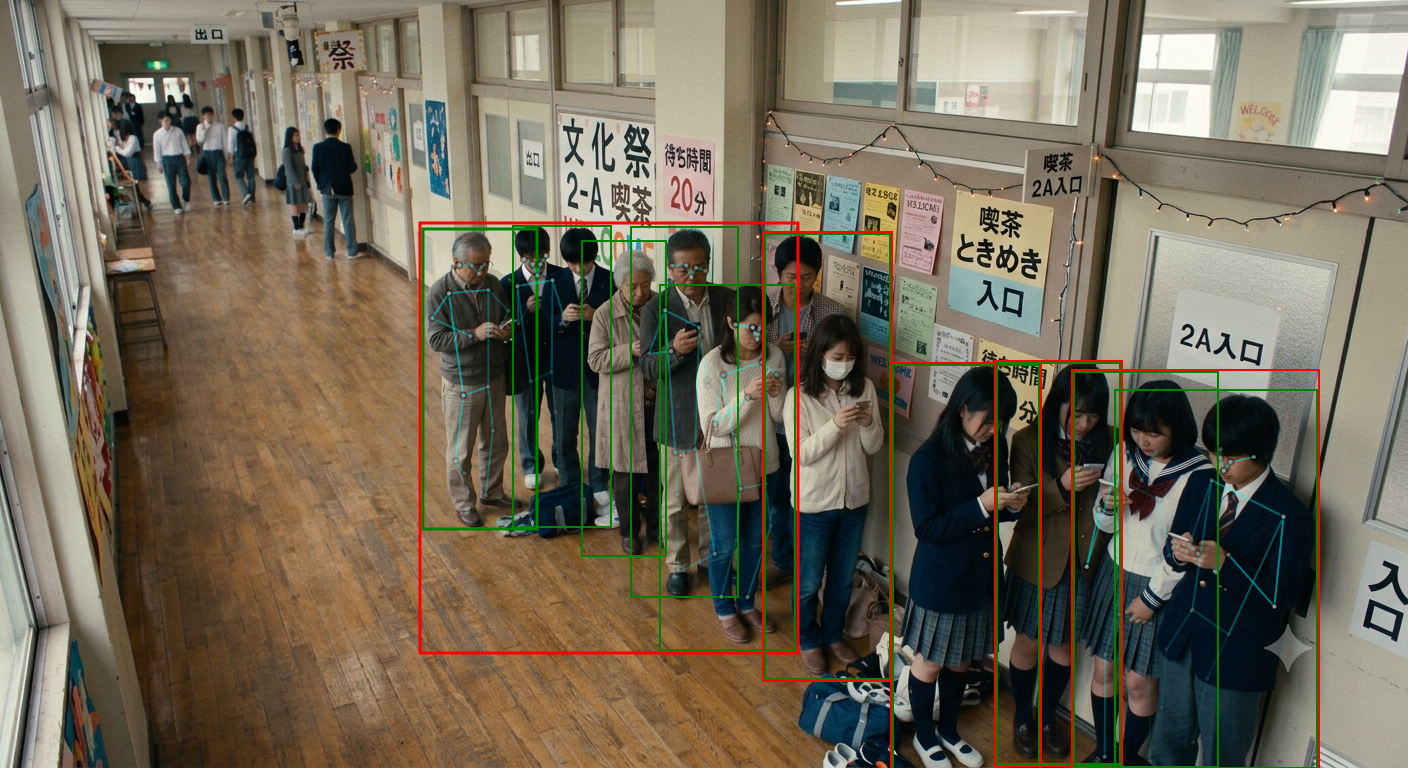
\includegraphics[width=0.25\textwidth]{experiment/results/approach_11_vector_orientation_grouping/strangers/detection_outputs/annotated_images/t_001s.png}}}$ &
      \jsonlen{experiment/results/approach_11_vector_orientation_grouping/strangers/detection_outputs/labels/t_001s.json} &
      % 符号と数値
        \ifnum\numexpr \jsonlen{experiment/results/approach_11_vector_orientation_grouping/strangers/detection_outputs/labels/t_001s.json} - \gtstrangers\relax>0 +\fi\the\numexpr
        \jsonlen{experiment/results/approach_11_vector_orientation_grouping/strangers/detection_outputs/labels/t_001s.json} - \gtstrangers\relax \\
    
    \hline
    
    $\vcenter{\hbox{視覚的クラッター}}$ &
      $\vcenter{\hbox{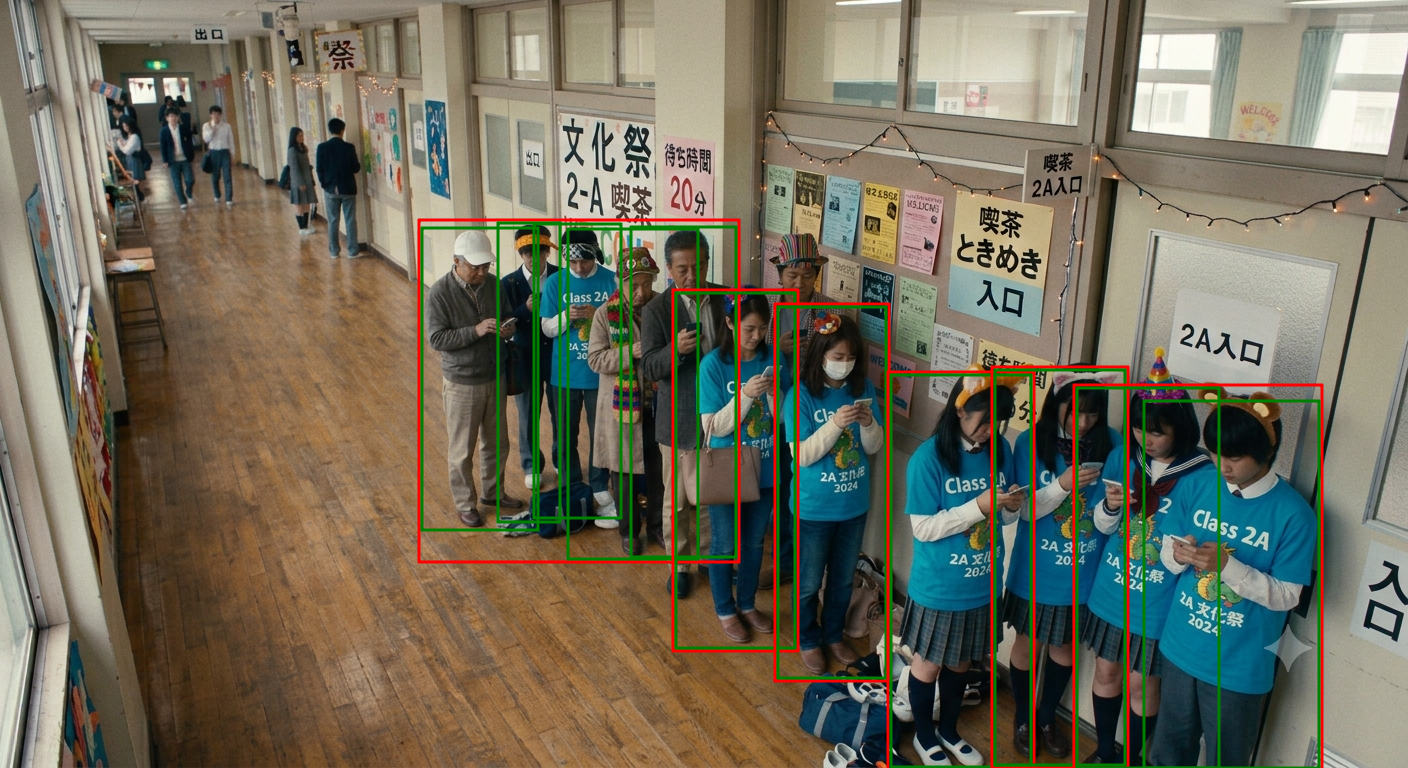
\includegraphics[width=0.25\textwidth]{experiment/results/approach_10_change_detection_model/various_clothes/detection_outputs/annotated_images/t_001s.png}}}$ &
      $\vcenter{\hbox{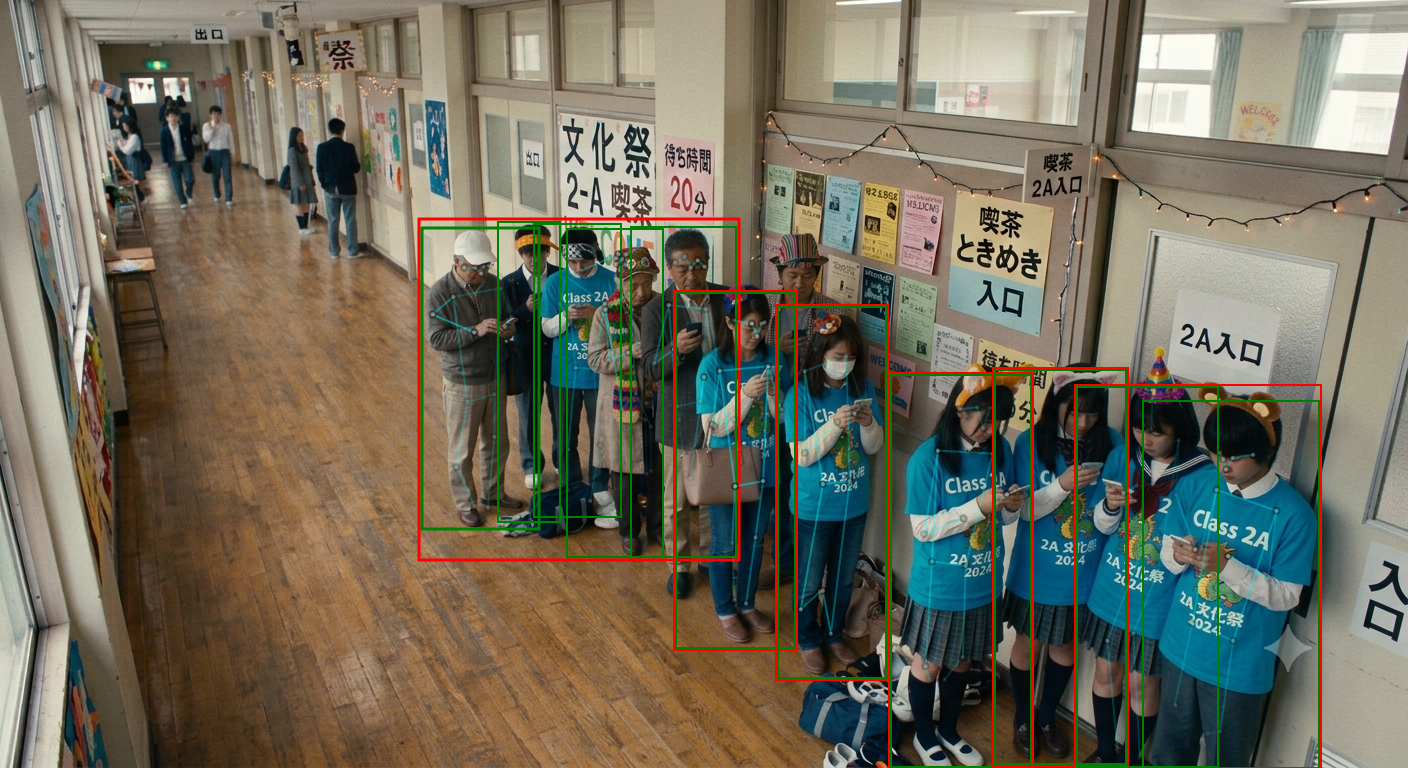
\includegraphics[width=0.25\textwidth]{experiment/results/approach_11_vector_orientation_grouping/various_clothes/detection_outputs/annotated_images/t_001s.png}}}$ &
      \jsonlen{experiment/results/approach_11_vector_orientation_grouping/various_clothes/detection_outputs/labels/t_001s.json} &
      % 符号と数値
        \ifnum\numexpr \jsonlen{experiment/results/approach_11_vector_orientation_grouping/various_clothes/detection_outputs/labels/t_001s.json} - \gtvariousclothes\relax>0 +\fi\the\numexpr
        \jsonlen{experiment/results/approach_11_vector_orientation_grouping/various_clothes/detection_outputs/labels/t_001s.json} - \gtvariousclothes\relax \\
    
    \hline

  \end{tabular}
  }
\end{table}

動画を入力データとして検証を行った際の実験結果を表\ref{tab:approach11_video_results}に示す。遮蔽物のない入力フレームおよびオクルージョン発生時のフレームを掲載している。

\begin{table}[H]
  \centering
  \small
  \caption{アプローチ11：実験結果の比較（動画）}
  \label{tab:approach11_video_results}
  \adjustbox{max width=\textwidth}{%
  \begin{tabular}{|c|c|c|c|c|}

    \hline

      & \begin{tabular}{c} 前アプローチの \\ 検出結果 \end{tabular}
      & 検出結果
      & \begin{tabular}{c} 検出された \\ グループ数 \end{tabular}
      & 実際のグループ数との差 \\
    
    \hline

    $\vcenter{\hbox{遮蔽物のない入力フレーム}}$ &
      $\vcenter{\hbox{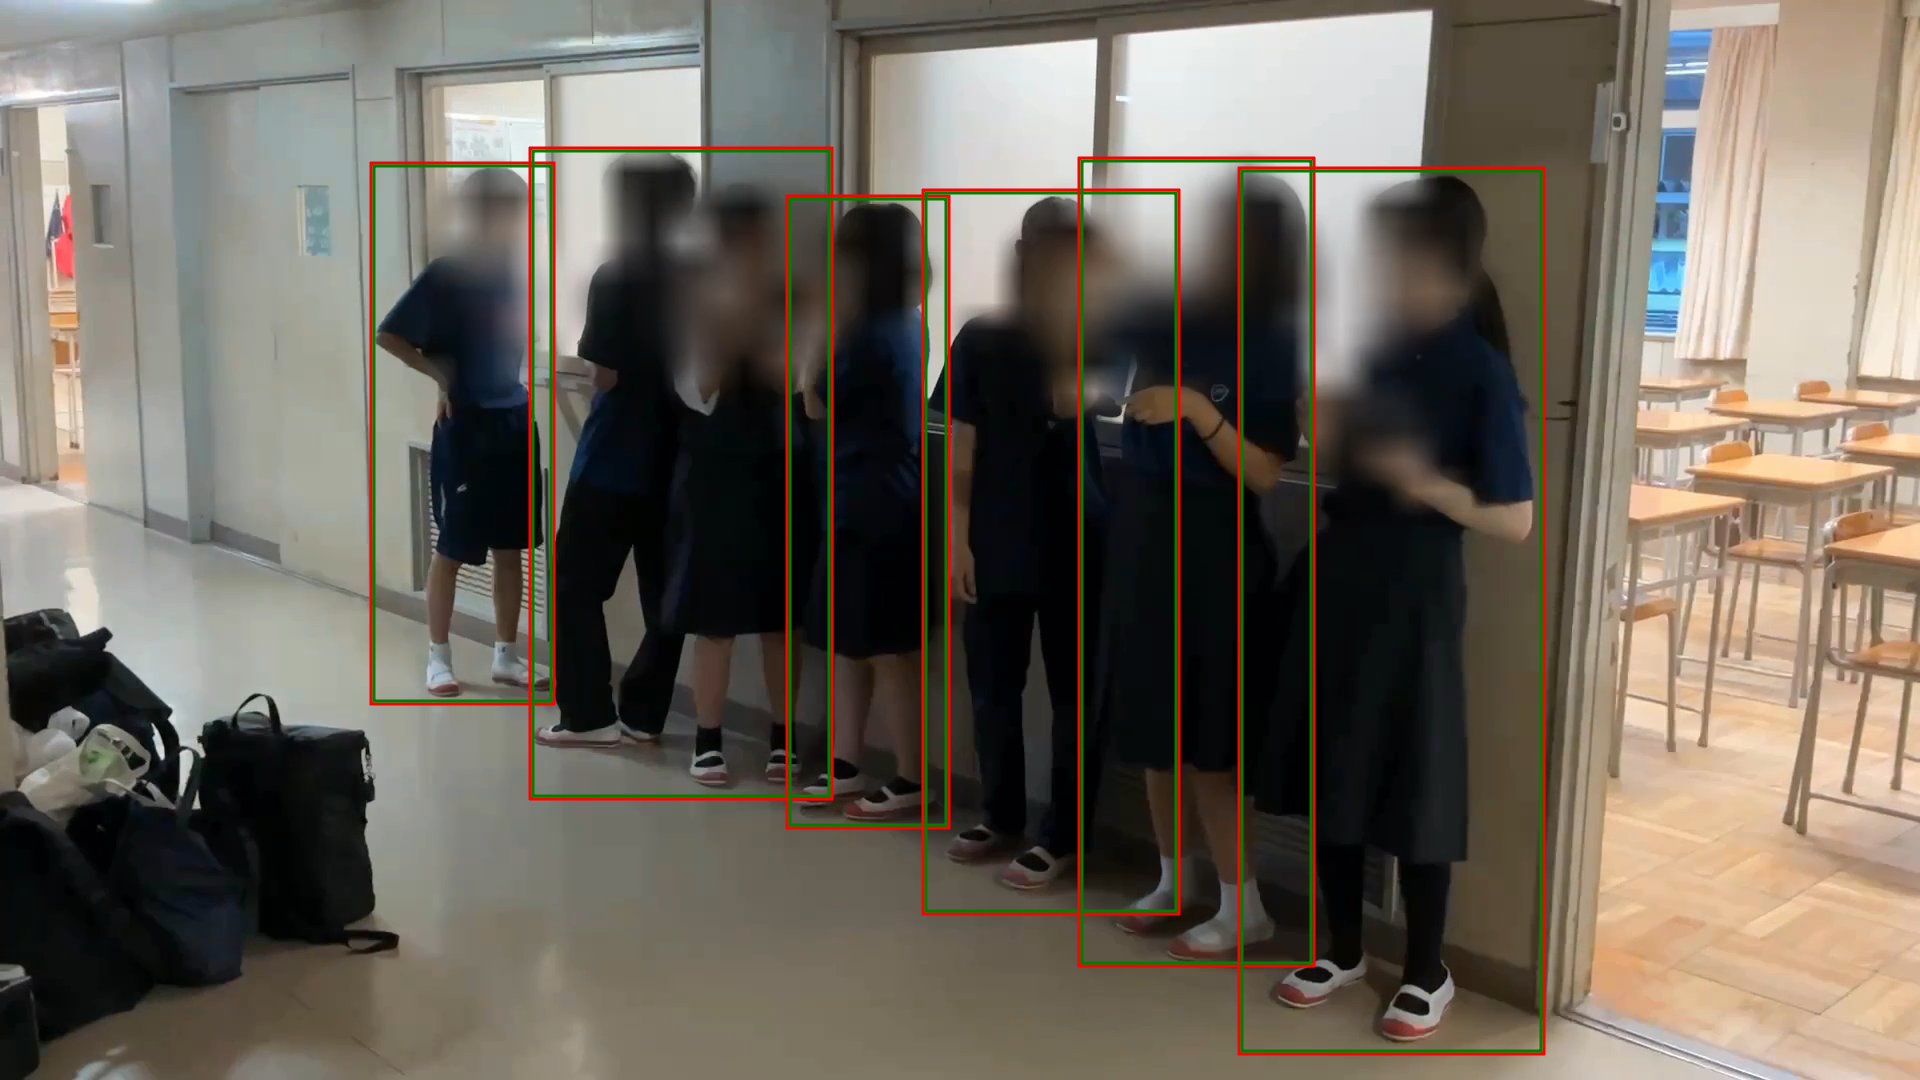
\includegraphics[width=0.25\textwidth]{experiment/results/approach_10_change_detection_model/queue_video/detection_outputs/annotated_images/t_012s.png}}}$ &
      $\vcenter{\hbox{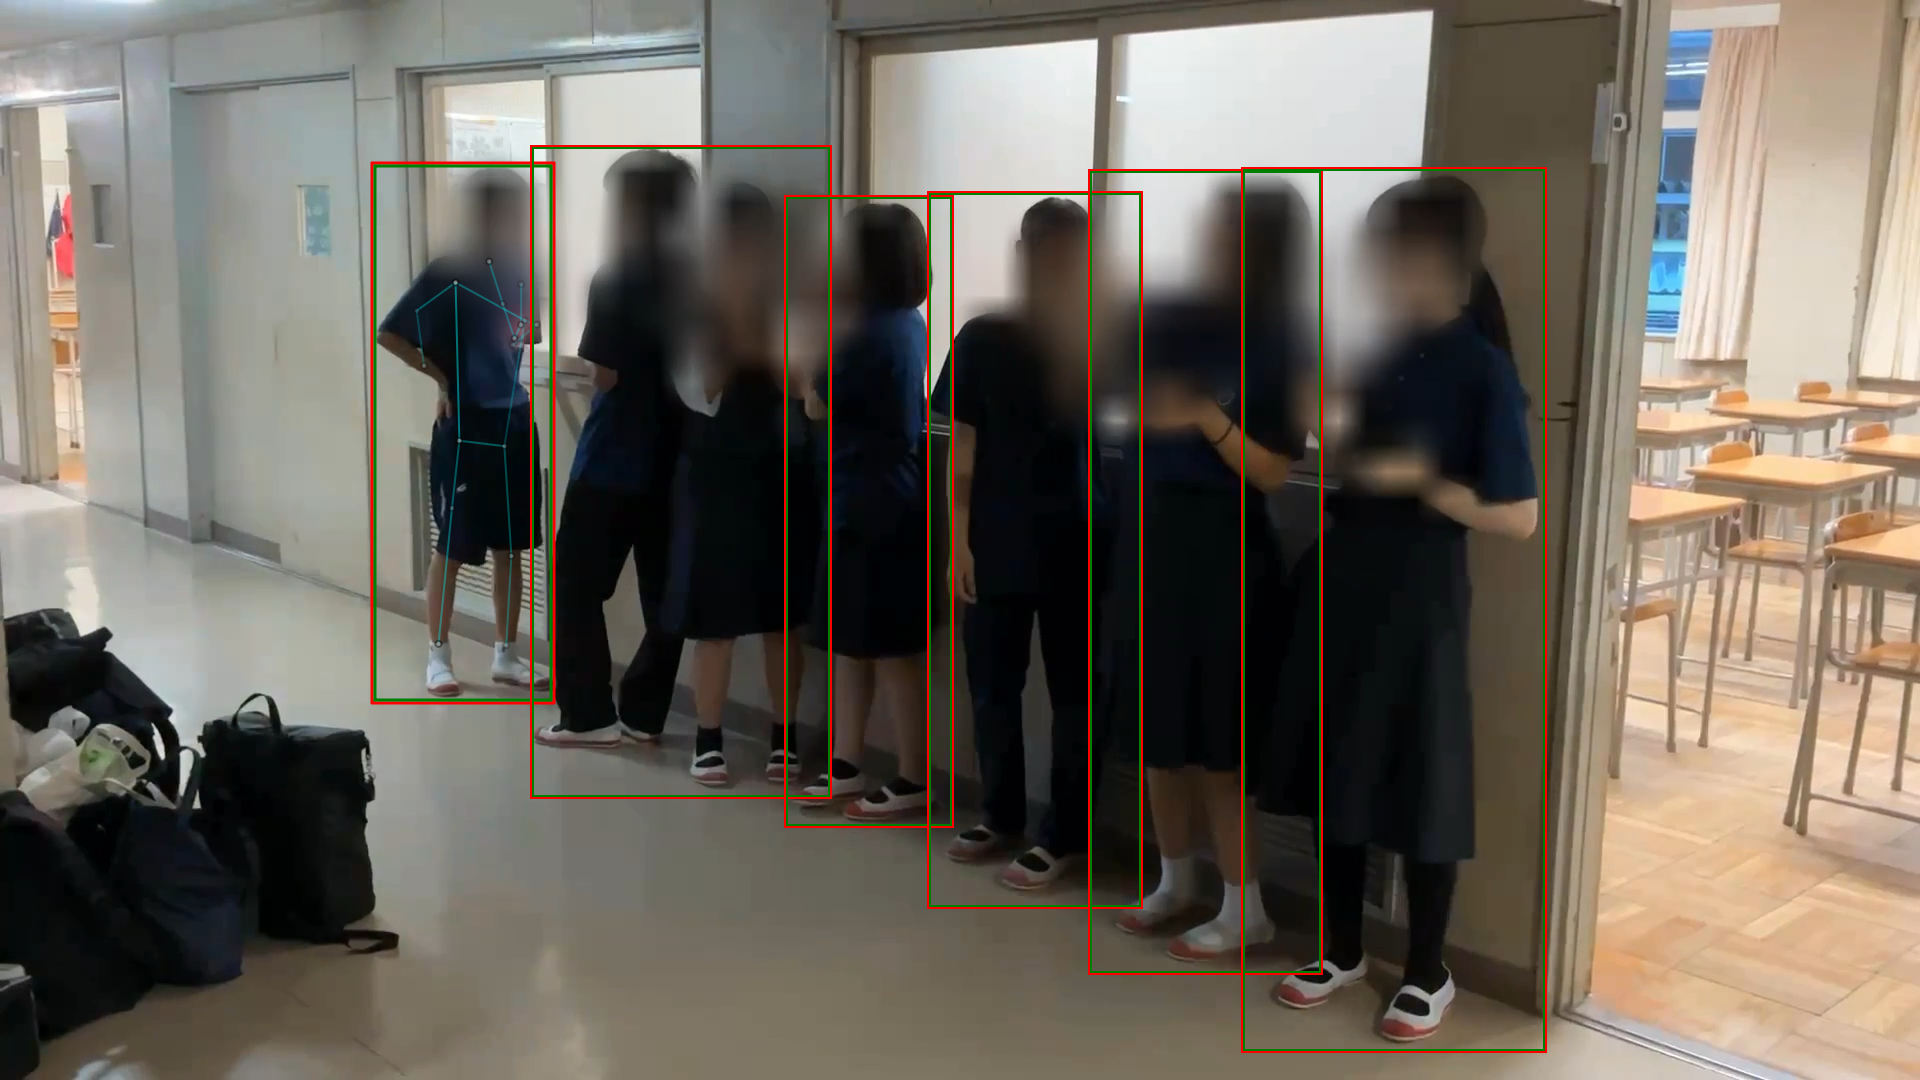
\includegraphics[width=0.25\textwidth]{experiment/results/approach_11_vector_orientation_grouping/queue_video/detection_outputs/annotated_images/t_012s.png}}}$ &
      \jsonlen{experiment/results/approach_11_vector_orientation_grouping/queue_video/detection_outputs/labels/t_012s.json} &
      % 符号と数値
        \ifnum\numexpr\jsonlen{experiment/results/approach_11_vector_orientation_grouping/queue_video/detection_outputs/labels/t_012s.json} - \gtvideoideal\relax>0 +\fi\the\numexpr
        \jsonlen{experiment/results/approach_11_vector_orientation_grouping/queue_video/detection_outputs/labels/t_012s.json} - \gtvideoideal\relax \\
    
    \hline
    
    $\vcenter{\hbox{オクルージョン発生時}}$ &
      $\vcenter{\hbox{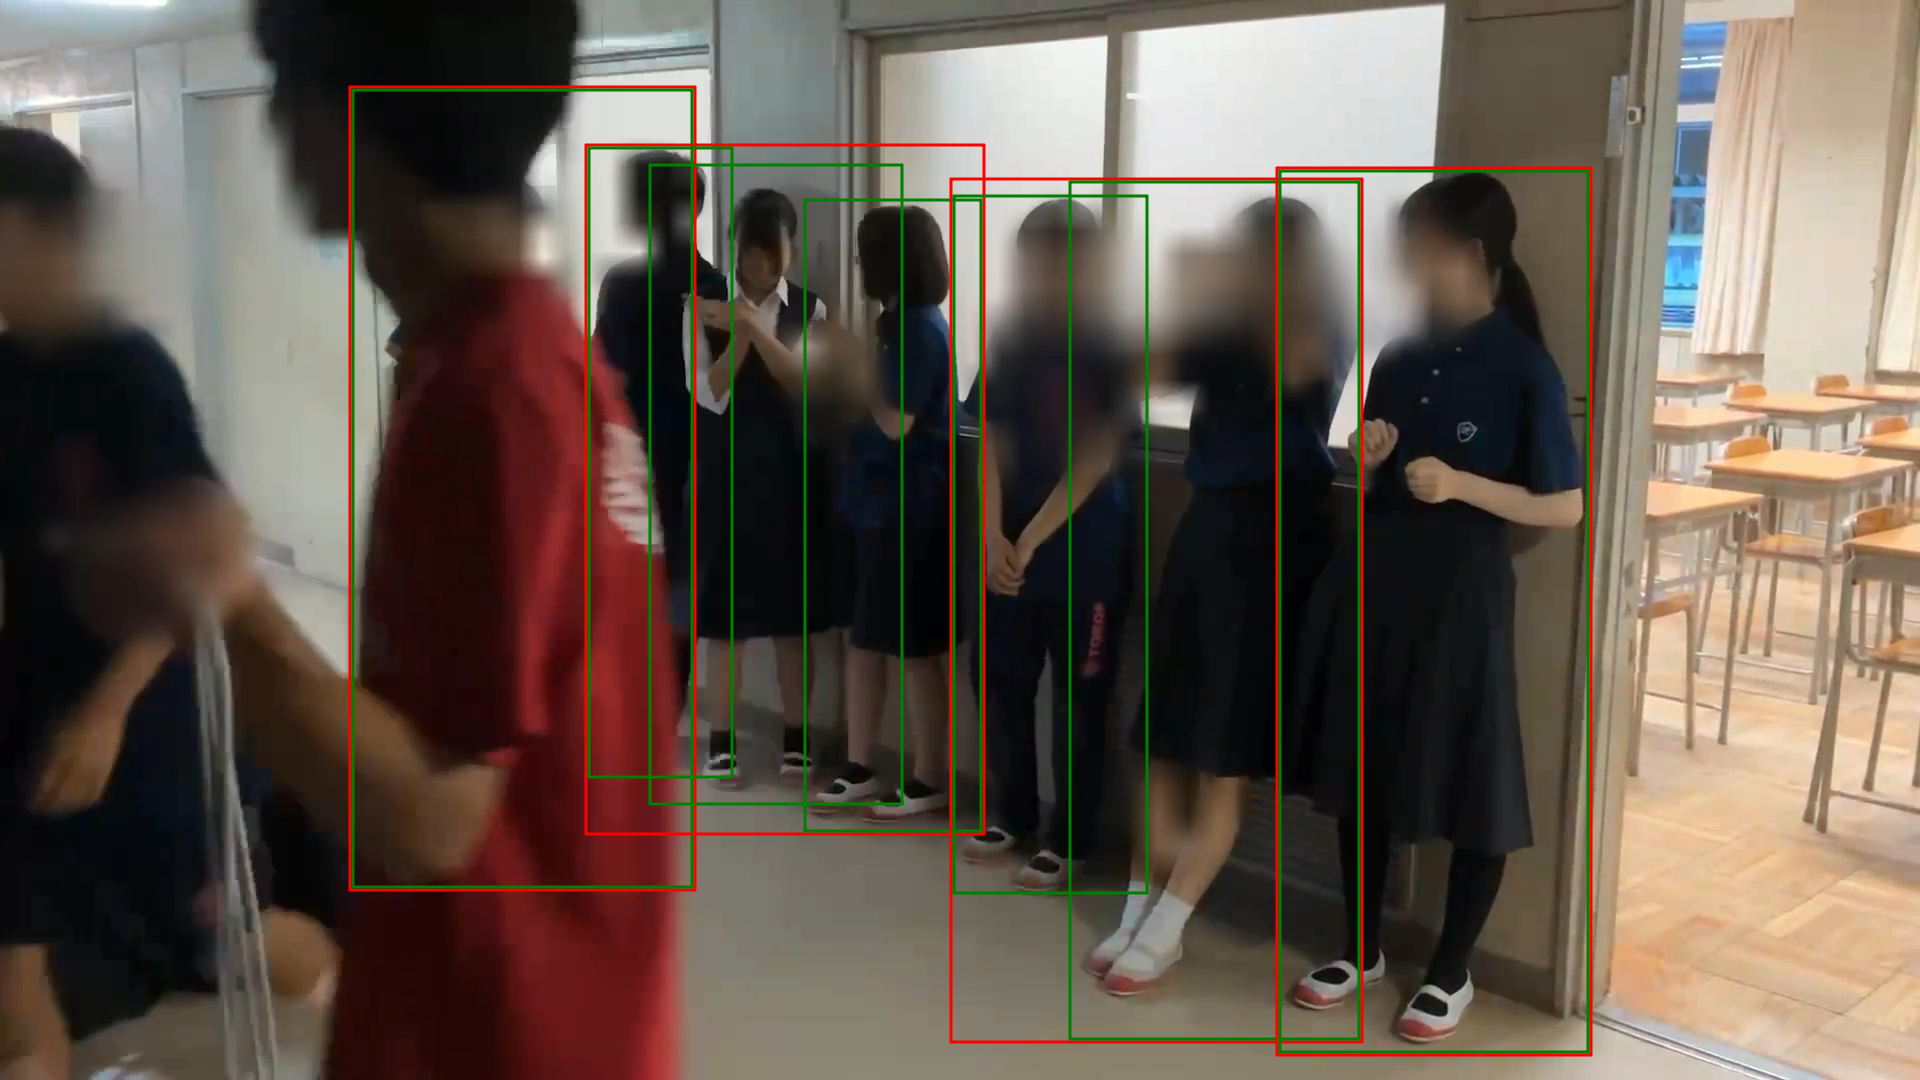
\includegraphics[width=0.25\textwidth]{experiment/results/approach_10_change_detection_model/queue_video/detection_outputs/annotated_images/t_017s.png}}}$ &
      $\vcenter{\hbox{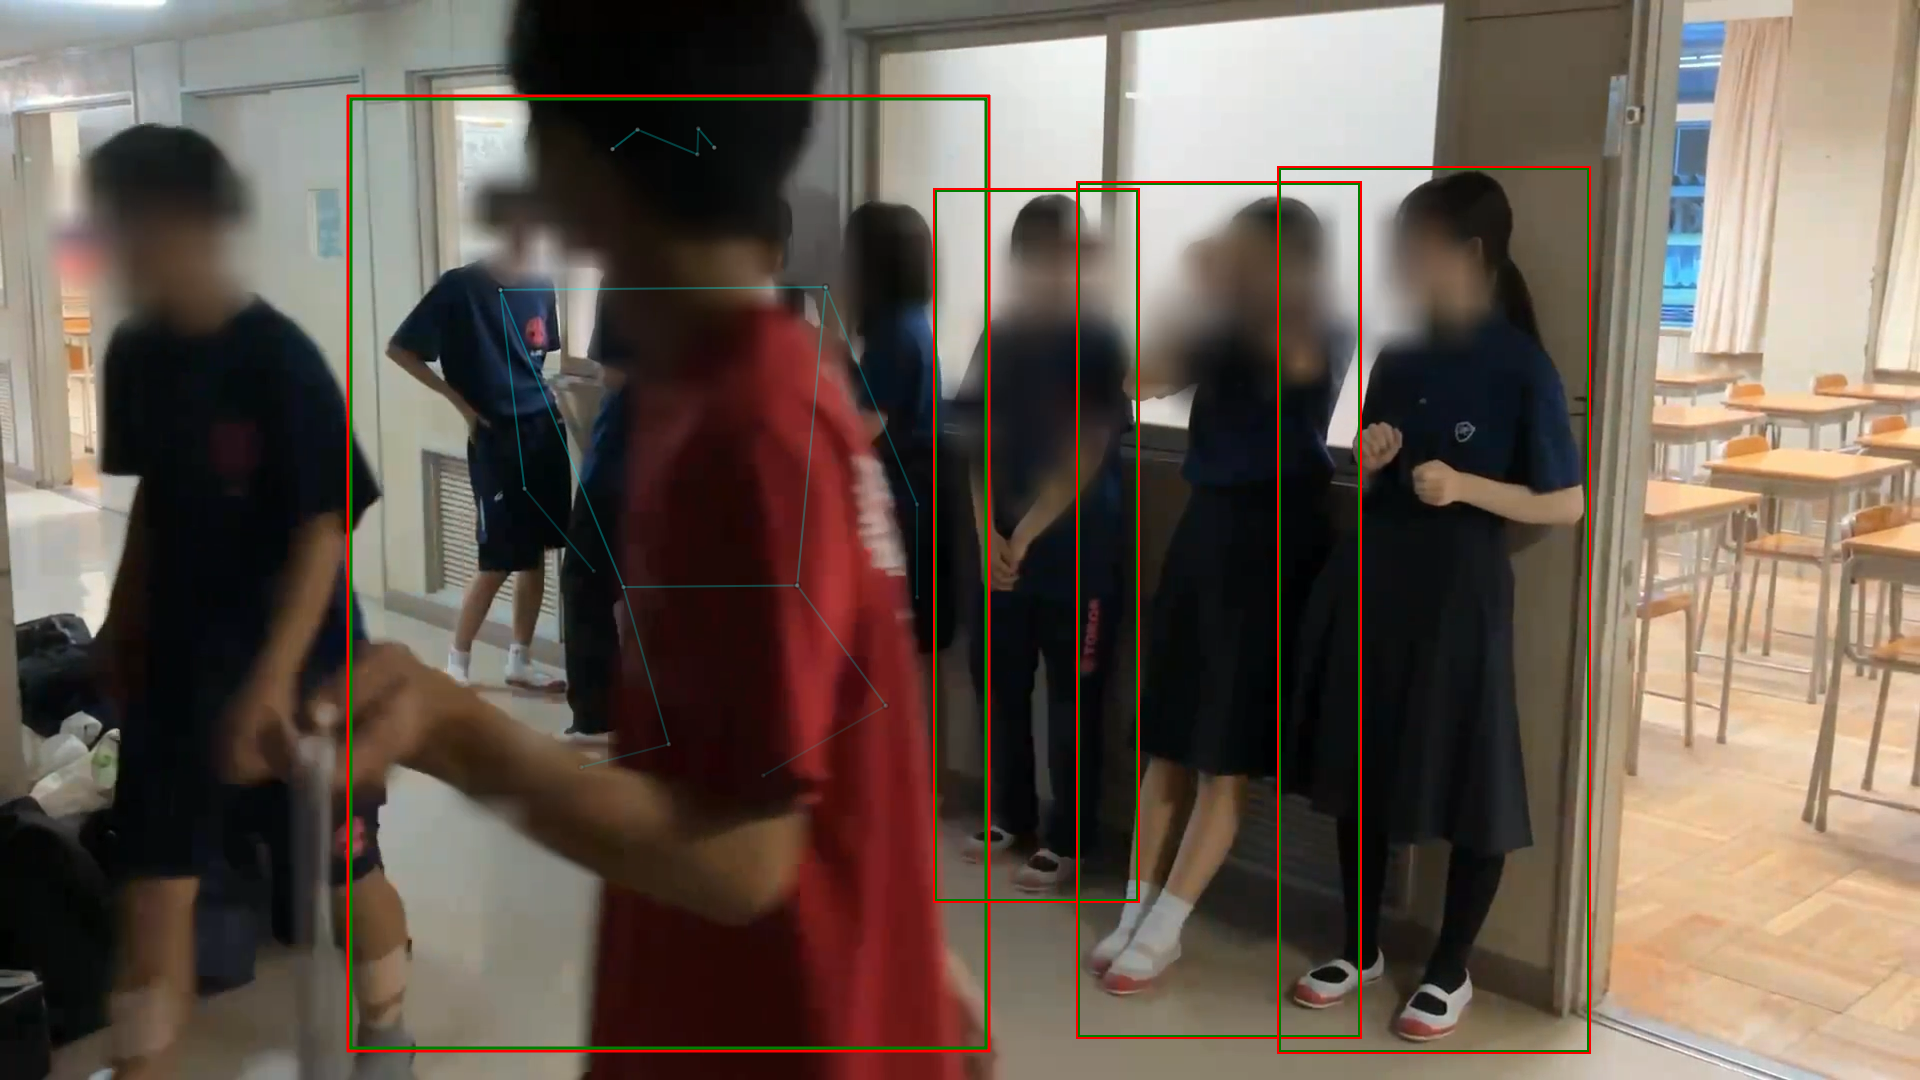
\includegraphics[width=0.25\textwidth]{experiment/results/approach_11_vector_orientation_grouping/queue_video/detection_outputs/annotated_images/t_017s.png}}}$ &
      \jsonlen{experiment/results/approach_11_vector_orientation_grouping/queue_video/detection_outputs/labels/t_017s.json} &
      % 符号と数値
        \ifnum\numexpr\jsonlen{experiment/results/approach_11_vector_orientation_grouping/queue_video/detection_outputs/labels/t_017s.json} - \gtvideoocclusion\relax>0 +\fi\the\numexpr
        \jsonlen{experiment/results/approach_11_vector_orientation_grouping/queue_video/detection_outputs/labels/t_017s.json} - \gtvideoocclusion\relax \\
    
    \hline
    
  \end{tabular}%
  }
\end{table}

\subsubsection{アプローチ10との比較}
距離ベースの並び判定に加え身体ベクトルの交差・距離閾値判定を導入したことで、前後の列に跨がって会話する人物群や斜めに向き合う連れ同士を正確に同一グループとして抽出可能となった。待機列内で自然に発生する多彩なコミュニケーション形態に対応した高精度なグループ化が実現された。

\subsection{課題}
アプローチ11において確認された課題は以下の通りである。

\begin{enumerate}
    \item \textbf{一時的な通過者（通行人）による誤検出}：
    単一フレームまたは短時間の情報のみで処理を行う場合、待機列の近傍を一時的に横切る通行人が特定の身体向きをとった際に、待機列内の構成員として誤ってグループに組み込まれるリスクが生じた。
\end{enumerate}

\clearpage
